\documentclass[journal, a4paper]{IEEEtran}

% some very useful LaTeX packages include:

%\usepackage{cite}      % Written by Donald Arseneau
                        % V1.6 and later of IEEEtran pre-defines the format
                        % of the cite.sty package \cite{} output to follow
                        % that of IEEE. Loading the cite package will
                        % result in citation numbers being automatically
                        % sorted and properly "ranged". i.e.,
                        % [1], [9], [2], [7], [5], [6]
                        % (without using cite.sty)
                        % will become:
                        % [1], [2], [5]--[7], [9] (using cite.sty)
                        % cite.sty's \cite will automatically add leading
                        % space, if needed. Use cite.sty's noadjust option
                        % (cite.sty V3.8 and later) if you want to turn this
                        % off. cite.sty is already installed on most LaTeX
                        % systems. The latest version can be obtained at:
                        % http://www.ctan.org/tex-archive/macros/latex/contrib/supported/cite/
\usepackage{amsfonts}
\usepackage{graphicx}   % Written by David Carlisle and Sebastian Rahtz
                        % Required if you want graphics, photos, etc.
                        % graphicx.sty is already installed on most LaTeX
                        % systems. The latest version and documentation can
                        % be obtained at:
                        % http://www.ctan.org/tex-archive/macros/latex/required/graphics/
                        % Another good source of documentation is "Using
                        % Imported Graphics in LaTeX2e" by Keith Reckdahl
                        % which can be found as esplatex.ps and epslatex.pdf
                        % at: http://www.ctan.org/tex-archive/info/

%\usepackage{psfrag}    % Written by Craig Barratt, Michael C. Grant,
                        % and David Carlisle
                        % This package allows you to substitute LaTeX
                        % commands for text in imported EPS graphic files.
                        % In this way, LaTeX symbols can be placed into
                        % graphics that have been generated by other
                        % applications. You must use latex->dvips->ps2pdf
                        % workflow (not direct pdf output from pdflatex) if
                        % you wish to use this capability because it works
                        % via some PostScript tricks. Alternatively, the
                        % graphics could be processed as separate files via
                        % psfrag and dvips, then converted to PDF for
                        % inclusion in the main file which uses pdflatex.
                        % Docs are in "The PSfrag System" by Michael C. Grant
                        % and David Carlisle. There is also some information
                        % about using psfrag in "Using Imported Graphics in
                        % LaTeX2e" by Keith Reckdahl which documents the
                        % graphicx package (see above). The psfrag package
                        % and documentation can be obtained at:
                        % http://www.ctan.org/tex-archive/macros/latex/contrib/supported/psfrag/

%\usepackage{subfigure} % Written by Steven Douglas Cochran
                        % This package makes it easy to put subfigures
                        % in your figures. i.e., "figure 1a and 1b"
                        % Docs are in "Using Imported Graphics in LaTeX2e"
                        % by Keith Reckdahl which also documents the graphicx
                        % package (see above). subfigure.sty is already
                        % installed on most LaTeX systems. The latest version
                        % and documentation can be obtained at:
                        % http://www.ctan.org/tex-archive/macros/latex/contrib/supported/subfigure/

\usepackage{url}        % Written by Donald Arseneau
                        % Provides better support for handling and breaking
                        % URLs. url.sty is already installed on most LaTeX
                        % systems. The latest version can be obtained at:
                        % http://www.ctan.org/tex-archive/macros/latex/contrib/other/misc/
                        % Read the url.sty source comments for usage information.

%\usepackage{stfloats}  % Written by Sigitas Tolusis
                        % Gives LaTeX2e the ability to do double column
                        % floats at the bottom of the page as well as the top.
                        % (e.g., "\begin{figure*}[!b]" is not normally
                        % possible in LaTeX2e). This is an invasive package
                        % which rewrites many portions of the LaTeX2e output
                        % routines. It may not work with other packages that
                        % modify the LaTeX2e output routine and/or with other
                        % versions of LaTeX. The latest version and
                        % documentation can be obtained at:
                        % http://www.ctan.org/tex-archive/macros/latex/contrib/supported/sttools/
                        % Documentation is contained in the stfloats.sty
                        % comments as well as in the presfull.pdf file.
                        % Do not use the stfloats baselinefloat ability as
                        % IEEE does not allow \baselineskip to stretch.
                        % Authors submitting work to the IEEE should note
                        % that IEEE rarely uses double column equations and
                        % that authors should try to avoid such use.
                        % Do not be tempted to use the cuted.sty or
                        % midfloat.sty package (by the same author) as IEEE
                        % does not format its papers in such ways.

\usepackage{amsmath}    % From the American Mathematical Society
                        % A popular package that provides many helpful commands
                        % for dealing with mathematics. Note that the AMSmath
                        % package sets \interdisplaylinepenalty to 10000 thus
                        % preventing page breaks from occurring within multiline
                        % equations. Use:
%\interdisplaylinepenalty=2500
                        % after loading amsmath to restore such page breaks
                        % as IEEEtran.cls normally does. amsmath.sty is already
                        % installed on most LaTeX systems. The latest version
                        % and documentation can be obtained at:
                        % http://www.ctan.org/tex-archive/macros/latex/required/amslatex/math/



% Other popular packages for formatting tables and equations include:

%\usepackage{array}
% Frank Mittelbach's and David Carlisle's array.sty which improves the
% LaTeX2e array and tabular environments to provide better appearances and
% additional user controls. array.sty is already installed on most systems.
% The latest version and documentation can be obtained at:
% http://www.ctan.org/tex-archive/macros/latex/required/tools/

% V1.6 of IEEEtran contains the IEEEeqnarray family of commands that can
% be used to generate multiline equations as well as matrices, tables, etc.

% Also of notable interest:
% Scott Pakin's eqparbox package for creating (automatically sized) equal
% width boxes. Available:
% http://www.ctan.org/tex-archive/macros/latex/contrib/supported/eqparbox/

% *** Do not adjust lengths that control margins, column widths, etc. ***
% *** Do not use packages that alter fonts (such as pslatex).         ***
% There should be no need to do such things with IEEEtran.cls V1.6 and later.


% Your document starts here!
\begin{document}
\begin{titlepage}

\newcommand{\HRule}{\rule{\linewidth}{0.5mm}} % Defines a new command for the horizontal lines, change thickness here

\center % Center everything on the page
 %----------------------------------------------------------------------------------------
%	LOGO SECTION
%----------------------------------------------------------------------------------------

~\\[1cm]

\includegraphics{SCUT.png}\\[2cm] % Include a department/university logo - this will require the graphicx package

%----------------------------------------------------------------------------------------
%	TITLE SECTION
%----------------------------------------------------------------------------------------

\HRule \\[1cm]
{ \huge \bfseries The Experiment Report of \textit{Machine Learning} }\\[0.6cm] % Title of your document
\HRule \\[2cm]
%----------------------------------------------------------------------------------------
%	HEADING SECTIONS
%----------------------------------------------------------------------------------------


\textsc{\LARGE \textbf{School:} School of Software Engineering}\\[1cm]
\textsc{\LARGE \textbf{Subject:} Software Engineering}\\[2cm] 

 
%----------------------------------------------------------------------------------------
%	AUTHOR SECTION
%----------------------------------------------------------------------------------------

\begin{minipage}{0.4\textwidth}
\begin{flushleft} \large
\emph{Author:}\\
Panan Wu % Your name
\end{flushleft}
\end{minipage}
~
\begin{minipage}{0.4\textwidth}
\begin{flushright} \large
\emph{Supervisor:} \\
Mingkui Tan % Supervisor's Name
\end{flushright}
\end{minipage}\\[2cm]
~
\begin{minipage}{0.4\textwidth}
\begin{flushleft} \large
\emph{Student ID:}\\
201630665908
\end{flushleft}
\end{minipage}
~
\begin{minipage}{0.4\textwidth}
\begin{flushright} \large
\emph{Grade:} \\
Undergraduate
\end{flushright}
\end{minipage}\\[2cm]

% If you don't want a supervisor, uncomment the two lines below and remove the section above
%\Large \emph{Author:}\\
%John \textsc{Smith}\\[3cm] % Your name

%----------------------------------------------------------------------------------------
%	DATE SECTION
%----------------------------------------------------------------------------------------

{\large \today}\\[2cm] % Date, change the \today to a set date if you want to be precise

 
%----------------------------------------------------------------------------------------

\vfill % Fill the rest of the page with whitespace

\end{titlepage}

% Define document title and author
	\title{Logistic Regression and Support Vector Machine}
	\maketitle

% Write abstract here
\begin{abstract}
In this experiment, I conduct two linear classifiers: logistic regression (LR) and support vector machine (SVM) using a9a dataset in LIBSVM Data. I evaluated the two methods mentioned above by plotting the loss value and accuracy during the parameters update process. Experimental results show that support vector machine converge faster than logistic regression and have higher accuracy on test sets, and  logistic regression's accuracy rate increase and loss value decrease are more stable and smooth than SVM.

\end{abstract}

% Each section begins with a \section{title} command
\section{Introduction}
	% \PARstart{}{} creates a tall first letter for this first paragraph
\PARstart{C}{lassifier} problem is a classical problem in machine learning. We have mutiple ways to solve these kind of problems, like logistic regression, support vector machine, decision tree, etc. The principle and ideas of each method are different, so the characteristics, efficiency and accuracy of classification methods are different. 

In this experiment, I implement two kinds of classification model: logistic regression and support vector machine. By plotting the loss of both training set and test set, and the accuracy of test set in training , we can intuitively know the differences between these two methods.

The motivations of this experiment are: (1) compare and understand the difference between gradient descent and batch random stochastic gradient descent, (2) compare and understand the differences and relationships between Logistic regression and linear classification and (3) further understand the principles of SVM and practice on larger data.

% Main Part
\section{Methods and Theory}

\subsection{Linear Classification}
 A linear classifier makes a classification decision based on the value of a linear combination of input features. 

Given training data ($\textbf{x}_i$; $y_i$) for i = 1...n, with $\textbf{x}_i \in \mathbb{R}^m$ and
$y_i \in \{-1,1\}$, learn a classfier f(\textbf{x}) such that:

$$ f(x)\left\{
\begin{aligned}
\geq 0& \quad    y_i = +1 \\
<0&  \quad y_i = -1 \\
\end{aligned}
\right.
$$

For a correct classification, $y_if(\textbf{x}_i) > 0$. And a linear classifier $f(\textbf{x})$ is:
$$f(\textbf{x})=\textbf{w}^T\textbf{x}+b$$.

In two-dimensional space, the discriminant is a line.
$\textbf{w}$ is the normal to the line, b is the bias. And \textbf{w} is known as the weight vector. While in three-dimensional space, the discriminant is a plane. In m-dimensional space, it becomes a hyperplane.

\subsection{Logistic Regression}

The logistic regression uses a logistic function to model a binary dependent variable. It outputs the likelihood of one class. And the logistic function is defined as: 
\begin{equation}
g(z) = \frac{1}{1+e^{-z}}
\end{equation} 
Our hypothesis is given by the combination of linear trasformation and logistic function:
\begin{equation}
h_\textbf{w}(\textbf{x}) = g(\sum_{i=1}^m w_ix_i) = g(\textbf{w}^T\textbf{x})
\end{equation}

And it represents the predict probability of true class. We cannot measure a probability. We can only see the occurence of an event and try to infer a
probability. And the probability we infered is described as:

\begin{equation}
P(y|\textbf{x}) = 
\left\{
\begin{aligned}
&h_\textbf{w}(\textbf{x}) \quad    &y = +1 \\
&1-h_\textbf{w}(\textbf{x})  \quad &y = -1 \\
\end{aligned}
\right.
\end{equation}

To evaluate our model, we use cross entropy error:

\begin{equation}
\textbf{E}_{in}(\textbf{w})= \frac{1}{n} \sum_{i=1}^nlog(1+e^{-y_n\cdot\textbf{w}^T\textbf{x}})
\end{equation}

It is based on an intuitive probabilistic interpretation of h. And it's very convenient and mathematically friendly (easy to minimize).

In order to keep the model simple and avoid overfitting, we introduce regularization into our loss function:

\begin{equation}
J(\textbf{w})= \frac{1}{n} \sum_{i=1}^nlog(1+e^{-y_n\cdot\textbf{w}^T\textbf{x}}) + \frac{\lambda}{2} ||\textbf{w}||^2_2
\end{equation}	

And the regularization parameter $\lambda$ a trade off between fitting the training set well and keeping the model relatively simple.

Conditional probabilities can be expressed in a different form to facilitate implementation:

\begin{equation}
P(y_i|\textbf{x}_i) = h_\textbf{w}(\textbf{x}_i)^{y_i}\cdot(1 - h_\textbf{w}(\textbf{x}_i))^{1-y_i}
\end{equation}	

And we can change loss function without regularization into another form:

\begin{equation}
J(\textbf{w})= \frac{1}{n}[ \sum_{i=1}^ny_ilogh_\textbf{w}(\textbf{x}_i)+(1-y_i)log(1-h_\textbf{w}(\textbf{x}_i))]
\end{equation}	

Then we calculate the gradient of the loss function to update our parameters:

\begin{equation}
\begin{aligned}
\frac{\partial J(\textbf{w})}{\partial\textbf{w}}
&= -\frac{1}{\partial \textbf{w}}\partial[ylogh_\textbf{w}(\textbf{x})+(1-y)log(1-h_\textbf{w}(\textbf{x}))] \\
&= (h_\textbf{w}(\textbf{x})-y)\textbf{x} \\
\end{aligned}
\end{equation}	

Now we can use gradient descent to update parameters according to the result of parital derivative:

\begin{equation}
\begin{aligned}
\textbf{w} := \textbf{w} -\frac{1}{n}\sum_{i=1}^{n} \alpha (h_\textbf{w}(\textbf{x}_i)-y_i)\textbf{x}_i
\end{aligned}
\end{equation}	

\subsection{Support Vector Machine}
The main idea of support vector machine (SVM) are to select two parallel hyperplanes that separate the two classes of data and let the distance between them as large as possible.
The region bounded by these two hyperplanes is called the "margin".

We first choose normalization such that $\textbf{w}^T \textbf{x}_+ + b = +1$ and $\textbf{w}^T \textbf{x}_- + b = -1$ for the positive and negative support vectors respectively. Then the magin is given by:

\begin{equation}
\frac{\textbf{w}}{||\textbf{w}||} \cdot (\textbf{x}_+-\textbf{x}_-) 
= \frac{\textbf{w}^T(\textbf{x}_+)-\textbf{x}_-}{||\textbf{w}||} 
= \frac{2}{||\textbf{w}||}
\end{equation}	

Learning the SVM can be formulated as an optimization:

\begin{equation}
\begin{aligned}
&\max_{\textbf{w},b} \frac{2}{||\textbf{w}||} \\
&s.t. \quad \textbf{w}^T\textbf{x}_i+b 
\left\{
\begin{aligned}
&\geq1 \quad    &y = +1 \\
&\leq-1  \quad &y = -1 \\
\end{aligned}
\right.
\end{aligned}
\end{equation}	

In general there is a trade off between the margin and the number of mistakes on the training data. Moreover, training data may not be linearly separable! Thus we introduce variable $\xi_i \geq 0$, for each i, which represents how much example i is on wrong side of margin boundary. If $\xi_i = 0$ then it is ok. If $ 0<\xi_i <1$ it is correctly classified, but with a smaller margin than $\frac{1}{||\textbf{w}||}$. If $\xi_i >1 $ then it is incorrectly classified.

So the optimization problem becomes:

\begin{equation}
\begin{aligned}
&\min_{\textbf{w},b} \frac{||\textbf{w}||^2}{2} + C \sum_{i=1}^n\xi_i \\
s.t. \quad &y_i(\textbf{w}^T\textbf{x}_i+b)\geq 1- \xi_i, \quad i=1,2...n
\end{aligned}
\end{equation}	

After that, we introduce hingle loss:

\begin{equation}
Hingle~loss = \xi_i = max(0, 1-y_i(\textbf{w}^T\textbf{x}_i+b))
\end{equation}	

And the optimization problem becomes:

\begin{equation}
\begin{aligned}
&\min_{\textbf{w},b} \frac{||\textbf{w}||^2}{2} + C \sum_{i=1}^n\xi_i \\
s.t. \quad &y_i(\textbf{w}^T\textbf{x}_i+b)\geq 1- \xi_i, \quad i=1,2...n
\end{aligned}
\end{equation}	

Since we finally have a good form of optimization problem, we now can compute the gradients:

\begin{equation}
\begin{aligned}
\frac{\partial f(\textbf{w},b)}{\textbf{w}} &= \textbf{w} + C\sum_{i=1}^{N}g_\textbf{w}(\textbf{x}_i) \\
\frac{\partial f(\textbf{w},b)}{b} &= C\sum_{i=1}^{N}g_b(\textbf{x}_i) \\
\end{aligned}
\end{equation}	

\section{Experiments}
\subsection{Dataset}

The dataset we used in this experiment is a9a dataset from LIBSVM Data. There are 32561 instances in the training dataset and 16281 instances in the test dataset. Both datasets have 123 features.

\subsection{Implementation}

\subsubsection{Logistic Regression}
.

First of all, I load the a9a dataset using $load\_svmlight\_file$ function in sklearn library. Since the dataset has already been splited into training set and test set, I just simply store data into different variables.

When it comes to initialize parameters. I choose to set all parameter into zero, initialize it randomly and with normal distribution separately to determine which one is the best. After that, I set learning rate to 0.2, batch size to 256, threshold to 0.5 and  update parameters. And then I calculate loss of both training set and validation set. I repeat this process 800 times and output the loss during each process.

Finally, I plot both training loss and validation loss during parameter update. As we can see from Fig.~\ref{fig:lr0}, the loss of validation set are stable decline. And then I plot the validation accuracy varing with the number of iterations, the accuracy of valiadation is stable increase. Finally, I output and plot the mean loss with different parameter initializers, as shown in TABLE~\ref{tab:lossInitial} and Fig.~\ref{fig:lr2}, the initializers in logistic regression have some impact on validation accuracy, and zero intializer seems to have the best effect on validation accuracy.

\begin{figure}[!hbt]
		\begin{center}
		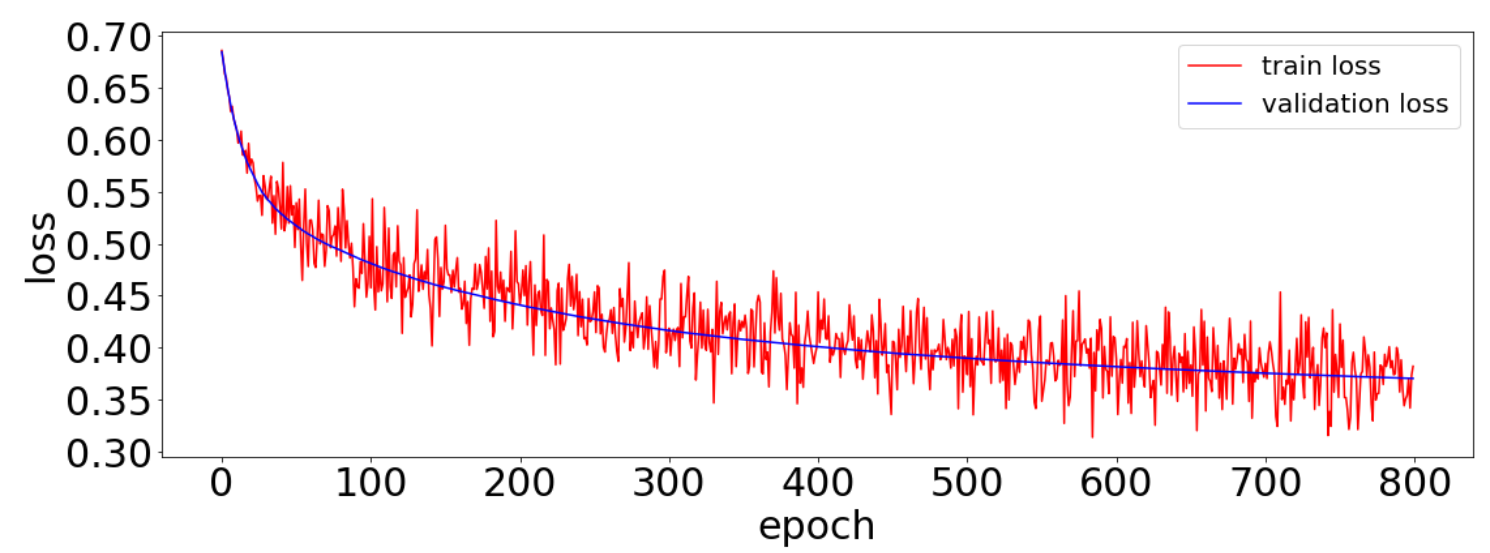
\includegraphics[width=\columnwidth]{lr0}
		\caption{The loss varing with the number of iterations.}
		\label{fig:lr0}
		\end{center}
	\end{figure}
	
	\begin{figure}[!hbt]
		\begin{center}
		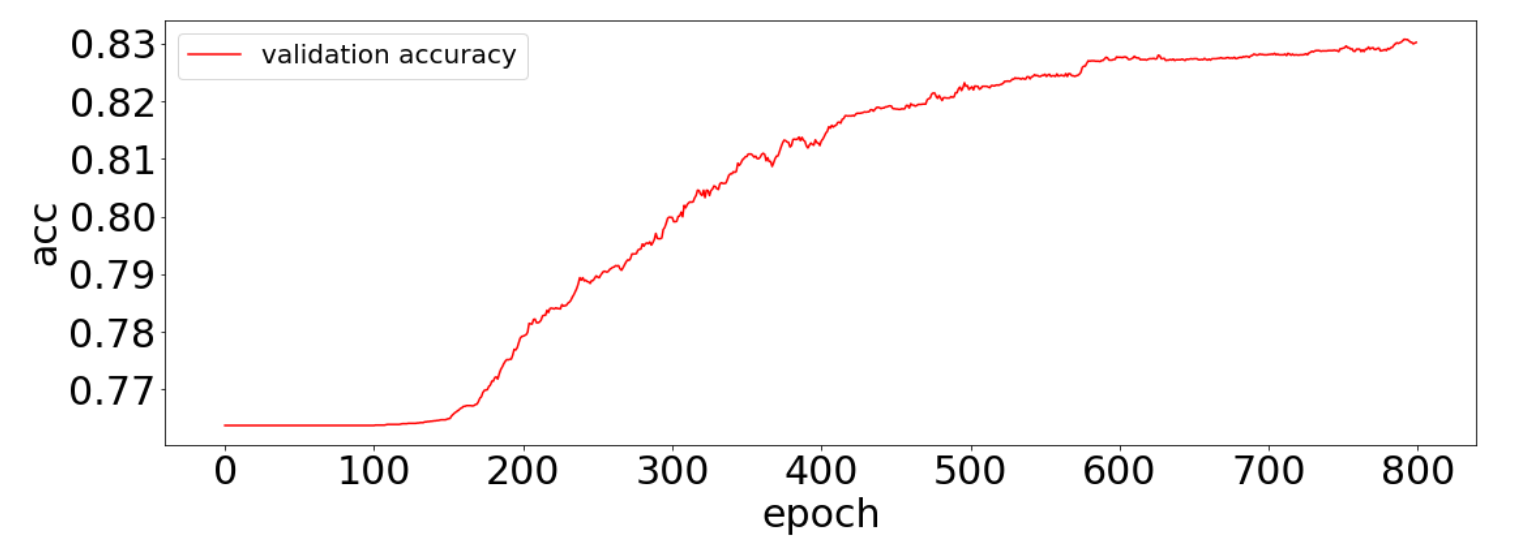
\includegraphics[width=\columnwidth]{lr1}
		\caption{The accuracy varing with the number of iterations.}
		\label{fig:lr1}
		\end{center}
	\end{figure}

	\begin{figure}[!hbt]
		\begin{center}
		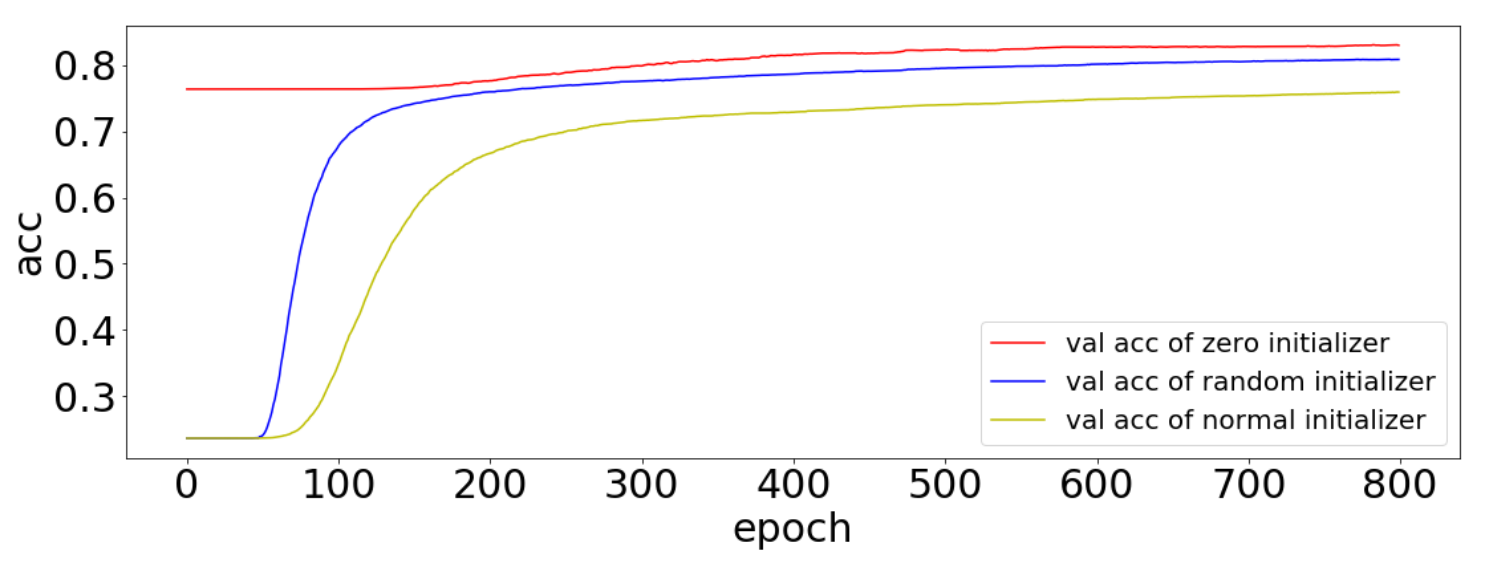
\includegraphics[width=\columnwidth]{lr2}
		\caption{The accuracy varing with the number of iterations and different intializers.}
		\label{fig:lr2}
		\end{center}
	\end{figure}
	
	\begin{table}[!hbt]
		\begin{center}
		\caption{Mean accuracy of last ten iterations with different initializer}
		\label{tab:lossInitial}
		\begin{tabular}{|c|c|}
			\hline
			Initializer & Mean Acc \\
			\hline
			Zero Initializer & 0.830 \\
			\hline
			Random Initializer & 0.809 \\
			\hline
			Normal Initializer & 0.759 \\
			\hline
		\end{tabular}
		\end{center}
	\end{table}



\subsubsection{Support Vector Machine}
.

As the same in logistic regression experiment, I read training data and test data into two variables. In training, I set learning rate to 0.005, soft margin trade off parameter C to 0.5 and max epoch to 100. I still try three types of parameter initializers. When it comes to parameters update, I first randomly choose 256 samples from training set and update parameters according to its partial derivative, and I calculate and store the training loss and validation loss with parameters just update.

As shown in Fig.~\ref{fig:svm0} and Fig.~\ref{fig:svm1}, the training loss and validation accuracy is unstable, but the validation loss is quite stable and keep declining. Different initializers still bring different mean  accuracy values, which means that choosing different initializers in svm will have a certain impact on the results.

	\begin{figure}[!hbt]
		\begin{center}
		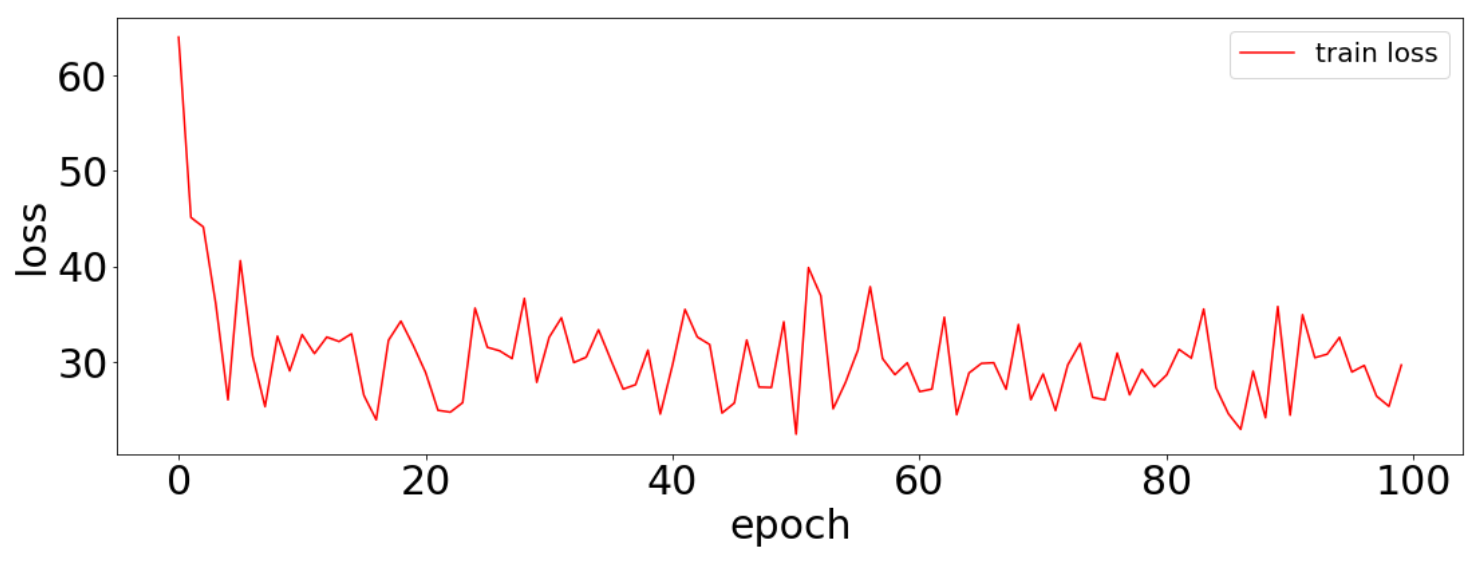
\includegraphics[width=\columnwidth]{svm0}
		\caption{The training loss varing with the number of iterations.}
		\label{fig:svm0}
		\end{center}
	\end{figure}
	
	\begin{figure}[!hbt]
		\begin{center}
		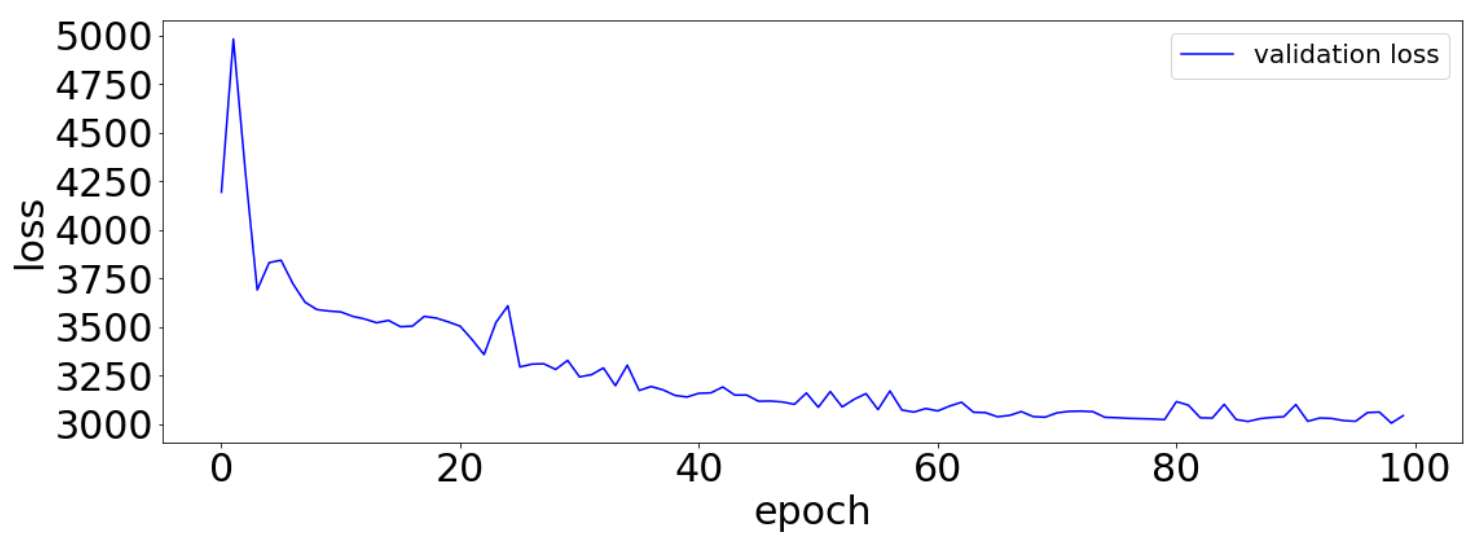
\includegraphics[width=\columnwidth]{svm1}
		\caption{The validation loss varing with the number of iterations.}
		\label{fig:svm1}
		\end{center}
	\end{figure}
	
	\begin{figure}[!hbt]
		\begin{center}
		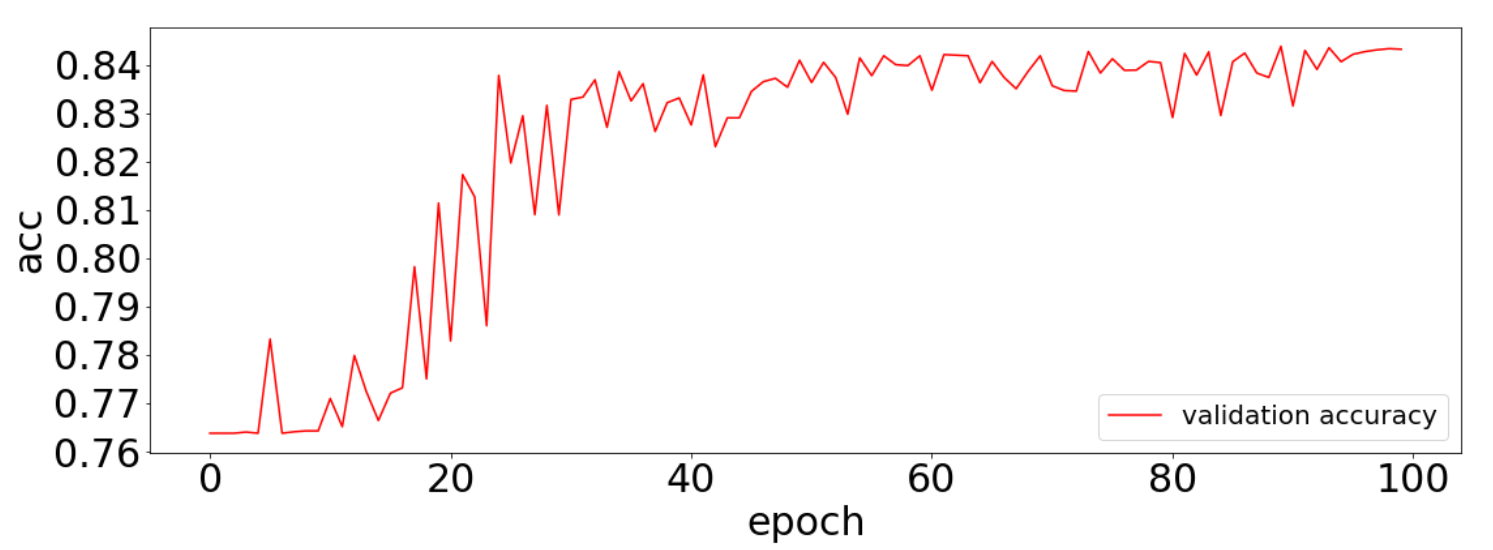
\includegraphics[width=\columnwidth]{svm2}
		\caption{The accuracy varing with the number of iterations.}
		\label{fig:svm2}
		\end{center}
	\end{figure}

	\begin{table}[!hbt]
		\begin{center}
		\caption{Mean accuracy with different initializer of last ten iterations}
		\label{tab:lossInitial1}
		\begin{tabular}{|c|c|}
			\hline
			Initializer & Mean Acc \\
			\hline
			Zero Initializer & 0.841 \\
			\hline
			Random Initializer & 0.842 \\
			\hline
			Normal Initializer & 0.827 \\
			\hline
		\end{tabular}
		\end{center}
	\end{table}

	\begin{figure}[!hbt]
		\begin{center}
		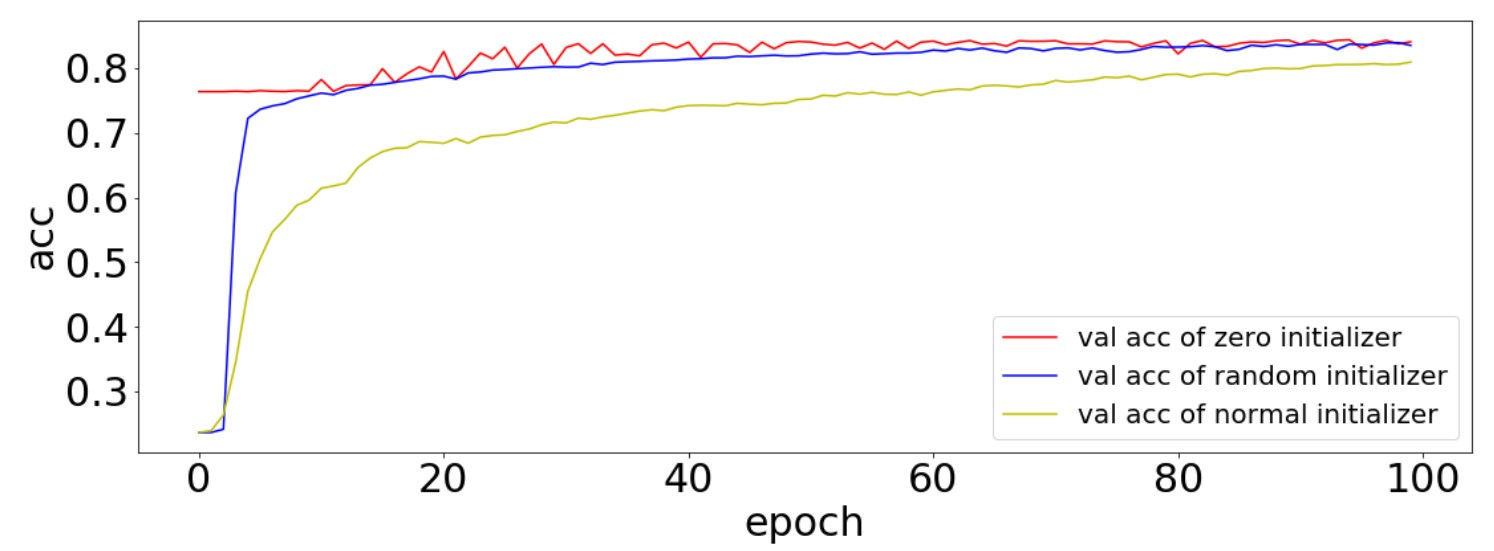
\includegraphics[width=\columnwidth]{svm3}
		\caption{The accuracy varing with the number of iterations and different intializers.}
		\label{fig:svm3}
		\end{center}
	\end{figure}
	
Finally, I compared the result of two methods mentioned above. We can know from Table~\ref{tab:acc} that support vector machine has higher validation accuracy than LR. And the number of iterations it needs are much lower than LR, the learning rate of SVM is much lower than LR too. But logistic regression has its own advantage, its validation set accuracy rate increase and loss value decrease are more stable and smooth than SVM. They both have four hyper-parameters that need to be artificially adjusted.

	\begin{table}[!hbt]
		\begin{center}
		\caption{Mean accuracy with different methods of last ten iterations}
		\label{tab:acc}
		\begin{tabular}{|c|c|}
			\hline
			Methods & Mean Acc \\
			\hline
			Logistic Regression & 0.842 \\
			\hline
			Support Vector Machine & 0.830 \\
			\hline
		\end{tabular}
		\end{center}
	\end{table}
	
\section{Conclusion}

In this experiment, I implement logistic regression and support vector machine, I analyse these two models mentioned above in different aspects and I make comparison between these two methods. From what has been shown above, we may safely draw the conclusion that support vector machine needs less iterations and lower learning rate than logistic regression, and the logistic regression's accuracy rate increase and loss value decrease are more stable and smooth than SVM. But we need to try other kinds of dataset to evalute these two methods better.

During this experiment, I realized what I learned in class, which enhanced my code practice ability. By comparing these two methods and writing experimental reports, I came into contact with a little scientific research. And it has increased my knowledge.

% Your document ends here!
\end{document}